%%%%%%%%%%%%%%%%%%%%%%%%%%%%%%%%%%%%%%%%%%%%%%
\section{Beamline instrumentations}
\label{sec:beaminstruments}

\subsection{Particle identification}


\subsubsection{Threshold Cherenkov counter}
The threshold Cherenkov counters have been used extensively in beamline to discriminate particles. Figure xyz shows one of the counters used in the CERN test beam area. It consists of a gas radiator that is contained in a long cylindrical tube, and a detection box in which the Cherenkov light is reflected by a 45$^\circ$ mirror and focused onto a photomultiplier tube. The diameter of the cylindrical tube is designed to allow the counter to pass through the standard CERN beam pile of about 20cm. A variety of gasses (e.g. CO2, nitrogen, argon, air, etc.) are available at CERN to optimize particle identification. The CERN beam group plans to install one thereshold Cherenkov counter in the H4 beamline. A second counter may be added to the beamline in additional funding is available.
\begin{cdrfigure}[CERN threshold Cherenkov counter]{ckv}{CERN threshold Cherenkov counter}
  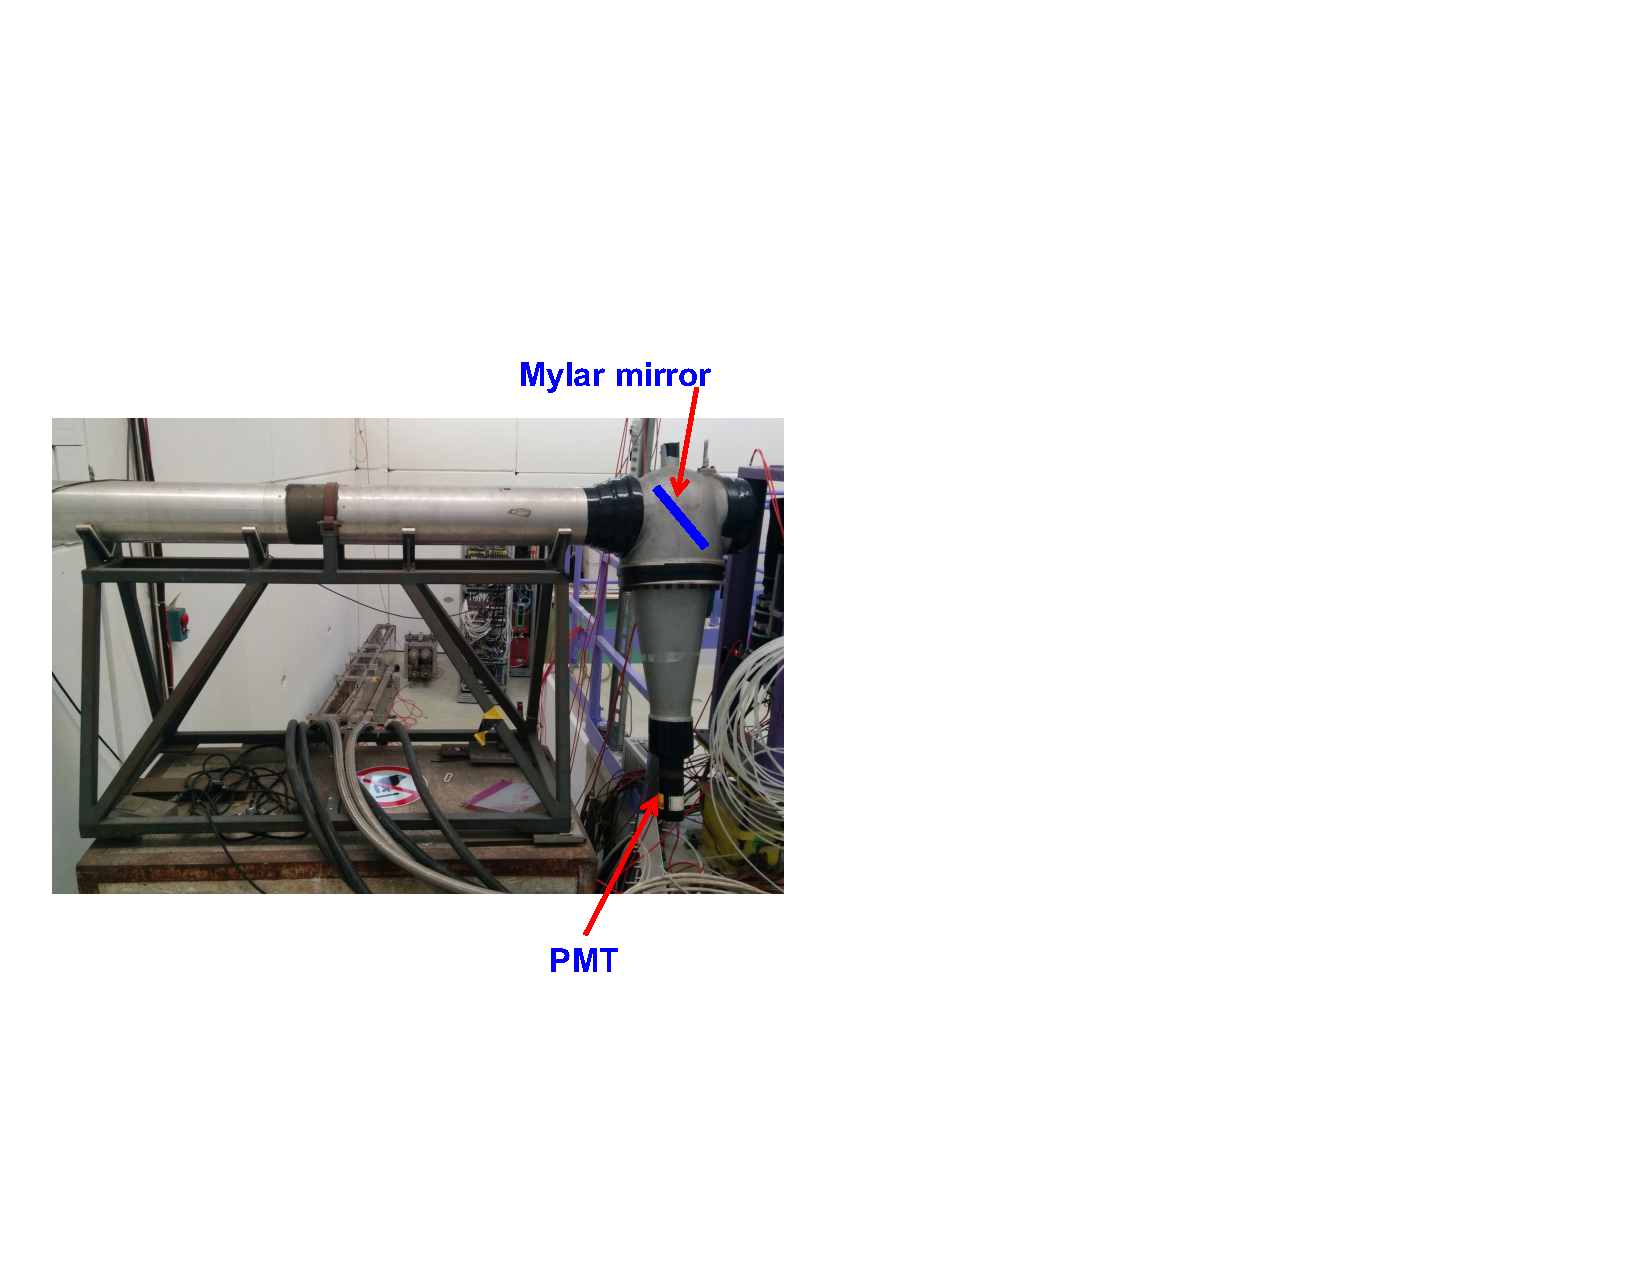
\includegraphics[width=0.65\textwidth]{beamline_ckv.pdf}
\end{cdrfigure}


\subsubsection{LAPPD Time-of-flight system}

\subsubsection{Other Time-of-flight system}

\subsection{Beam profile and particle tracking}

\subsubsection{Fiber tracker}

\subsubsection{Multiwire Proportional Chambers}

\subsection{Momentum measurements}

\subsubsection{Spectrometer}

\subsubsection{Beam collimation}

\subsection{DAQ and Trigger}

\subsubsection{Interface with artDAQ}

\subsubsection{Interface with Trigger Board}





